\documentclass[11pt]{article}
\usepackage{listings} % Required for Code
\usepackage[left = 1cm, right = 1cm, top = 1cm, bottom = 2cm]{geometry} % Set margins
\usepackage{amsmath} % Required for Writing Mathematics
\usepackage{amssymb} % Contains some mathematical symbols
\usepackage{amsthm}
\usepackage{mathtools}
\DeclarePairedDelimiter\ket{\lvert}{\rangle}
\usepackage{amsfonts} % Contains some mathematical fonts
\usepackage{siunitx}
\usepackage{float} % you insert figures into "floats"
\usepackage{subcaption}
\usepackage[skip=2pt,font=scriptsize]{caption} % added captions
\usepackage{graphicx}

\setlength{\parindent}{0pt} % no paragraph indent
\setlength{\parskip}{\medskipamount} % changes paragraph skip

\DeclareMathOperator{\sech}{sech}
\DeclareMathOperator{\csch}{csch}


\title{Electromagnetic Waves - Adil Hashlamon - 6813102}
\author{Adil Hashlamon}
\date{December 2024}
\begin{document}
\underline{\textbf{Example Sheet 1 Worked Solutions}}

\underline{Question 1}

\textit{Question.} Establish Stirling's Formula: $N \approx \sqrt{2\pi N }N^N e^{-N}$

\begin{proof}
We are first given $\int\limits_{0}^{\infty}e^{-x} x^N dx = \int\limits_{0}^{\infty}e^{-F(x)} dx$ and since the integrands are equal, we can equate:
\begin{equation}
    \begin{aligned}
        e^{-x}x^N &= e^{-F(x)} \\
        \Rightarrow F(x) &= x - N\ln x.
    \end{aligned}
\end{equation}

We then differentiate twice in order to find the approximation $F(x) \approx F(x_0) + F''(x_0) (x-x_0)^2/2$ where $x_0$ is $x$ value of the minimum of $F(x)$.
\begin{equation}
    \begin{aligned}
        F'(x) &= 1- \frac{N}{x} \\
        F''(x) &= \frac{N}{x^2}.
    \end{aligned}
\end{equation}

The minimum occurs when $F'(x)=0$ which implies $x_0 = N$ (we assume this is a minimum as it is the only solution to $F'(x)=0$ and the question asks us to find a minimum).

We know have all the information required to determine the approximation and can substitute into the 2nd integral given:

\begin{equation}
    F(x) \approx -N + N \ln  N - \frac{(x-N)^2}{2N}
\end{equation}

\begin{equation}
    \begin{aligned}
        N! &= \int\limits_{0}^{\infty} \exp\left(-N + N \ln  N - \frac{(x-N)^2}{2N}\right) dx \\
        & = e^{-N} N^N \int\limits_{0}^{\infty} \exp\left( - \frac{(x-N)^2}{2N}\right) dx.
    \end{aligned}
\end{equation}

The time has come to apply the final approximation alluded to in the question. The term $x-N$ is effectively shifting the function to the right hand side of the y-axis. And since $N$ is very large, the limits of the integral guarantee that we are integrating the entire curve as it tails to $0$ at either end. \textit{Note: }The factor of $1/2N$ does effectively nothing to affect this shifting.

\begin{figure}[H]
\centering 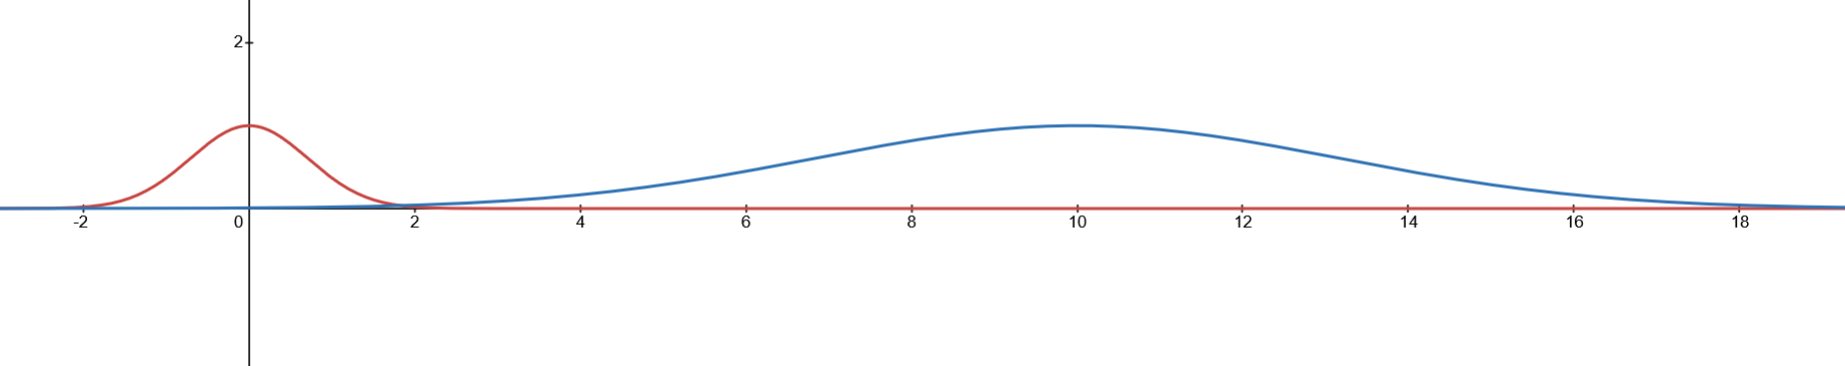
\includegraphics[scale=0.4]{Question 1.1.png} \label{fig:FFTgen}
\caption{Graph of $\exp{-x^2}$ in red vs $\exp(-{(x-10)^2}/{20})$ in blue}
\end{figure}
\newpage
Thus, we make the approximation:
\begin{equation}
    N! \approx e^{-N} N^N \int\limits_{-\infty}^{+\infty} \exp\left(\frac{-x^2}{2N}\right) dx.
\end{equation}

As this is the standard form of the Gaussian Integral:
\begin{equation}
    \int\limits_{-\infty}^{+\infty}e^{-ax^2} dx = \sqrt{\frac{\pi}{a}}.
\end{equation}

Thus, with $a= 1/2N$, we have:

\begin{equation}
    N! \approx \sqrt{2\pi N} N^N e^{-N}
\end{equation}
    
\end{proof}


\underline{Question 2i}

\textit{Question.} For a two coupled system in the microcanonical ensemble, show that they maximise their entropy if the heat capacity, $C$, is positive.

\begin{proof}
Considering the system as a whole to have entropy $S$ and equal temperature $T$, we have the equation:
\begin{equation}
    \frac{\partial^2S}{\partial E^2} = -\frac{1}{T^2C}
\end{equation}
If we want the system to have a maximum entropy, the equation on the right hand side must be negative and thus $C$ must be positive.

\end{proof}

\underline{Question 2ii}

\textit{Question.} Show that the energy fluctuations $\triangle E^2 = \langle E^2 \rangle - \langle E\rangle ^2$ are proportional to $C_V$ in the canonical ensemble.


\begin{proof}
    The fluctuations in the canonical ensemble can be written as: 
    \begin{equation}
        \triangle E^2 = - \frac{\partial \langle E \rangle}{\partial \beta}
    \end{equation}
    The definition of the heat capacity $C_V$ in this case is given as: 
    
    \begin{equation}
        \begin{aligned}
            C_V &= \left(\frac{\partial \langle E \rangle}{\partial T} \right)_V \\
            \Rightarrow \partial \langle E \rangle &= C_V \cdot \partial T \\
            \Rightarrow \triangle E^2 &= - C_V \cdot \frac{\partial T}{\partial \beta}
        \end{aligned}
    \end{equation}
    where the subscript denotes that the volume is constant.

    By definition:
    \begin{equation}
            \begin{aligned}
                \beta &= \frac{1}{k_BT}, T\neq 0 \\
                \Rightarrow \frac{\partial \beta}{\partial T} &= - \frac{1}{k_BT^2} \\
                \Rightarrow \frac{\partial T}{\partial \beta} &= -k_BT^2, T\neq 0 \\
                \Rightarrow \triangle E^2 &= C_V k_B T^2, T \neq 0
            \end{aligned}
    \end{equation}
    
\end{proof}

\underline{Question 2iii}

\textit{Question.} Show that the Gibbs entropy from the canonical ensemble can be written as 
\begin{equation}
    S = k_B \frac{\partial}{\partial T}(T\ln Z)
\end{equation}
\begin{proof}
    The entropy in the canonical system, derived using the standard definition of $S$ and Stirlings formula is given as:
    \begin{equation}
        S = - k_B \sum_n p(n) \ln p(n).
    \end{equation}

    The probability of the system being in a state $\ket{n}$ is given by the Boltzmann distribution:
    \begin{equation}
        p(n)= \frac{e^{-\beta E_n}}{Z}
    \end{equation}

    Substituting into our form of S:
    \begin{equation}
        \begin{aligned}
            S &= -k_B \sum_n \frac{e^{-\beta E_n}}{Z} \ln \left(\frac{e^{-\beta E_n}}{Z}\right) \\
            &= - k_B \sum_n \frac{e^{-\beta E_n}}{Z} \left[-\beta E_n - \ln Z\right] \\
            &= k_B \sum_n \frac{\beta E_ne^{-\beta E_n}}{Z} + \frac{e^{-\beta E_n}}{Z} \ln Z \\
            &= k_B \left[ \sum_n \frac{\beta E_n}{Z} e^{-\beta E_n} + \ln Z\right],
        \end{aligned}   
    \end{equation}
Where the last step is made as $\sum_n e^{-\beta E_n}/Z = \sum_n p(n) =1$ as something must happen.

Now, we work backwards from the Gibbs entropy:
\begin{equation}
    \begin{aligned}
        S &= k_b \frac{\partial}{\partial T} (T \ln Z) \\
        & = k_B \left[T \cdot \frac{1}{Z} \cdot \frac{\partial Z}{\partial T} + \ln Z\right]
    \end{aligned}
\end{equation}

$Z$ is given as: 
\begin{equation}
    \begin{aligned}
        Z &= \sum_n e^{-\beta E_n} \\
        &= \sum_n e^{-E_n/k_BT}
    \end{aligned}
\end{equation}

Differentiating with respect to T:
\begin{equation}
    \begin{aligned}
        \frac{\partial Z}{\partial T} &= \sum \frac{\partial}{\partial T} (e^{-E_n/k_BT})\\
        &= \sum_n \frac{\partial }{\partial T} \left(- \frac{E_n}{k_BT} \right)e^{- E_n/k_B T}\\
        &= \sum_n \frac{E_n}{k_B T^2} e^{-E_n/k_BT} \\
        &= \sum_n \frac{E_n}{k_B T^2} e^{-\beta E_n}.
    \end{aligned}
\end{equation}
\newpage
We can now substitute this into the Gibbs entropy equation:
\begin{equation}
    \begin{aligned}
        S &= k_B \left[\frac{T}{Z} \sum_n \frac{E_n}{k_B T^2} e^{-\beta E_n} + \ln Z\right] \\
        &= k_B \left[ \sum_n \frac{\beta E_n}{Z} e^{-\beta E_n} + \ln Z\right] \\
        & = k_B \frac{\partial}{\partial T} (T \ln Z)        
    \end{aligned}
\end{equation}
\end{proof}

\underline{Question 3}

\textit{Question.} In a system of $N$ spin $1/2$ particles, each with energy of $\pm \mu B/2$ where $\mu$ is the magnetic moment, show that the partition function is
\begin{equation}
    Z = 2^N \cosh^N\left(\frac{\beta \mu B}{2}\right),
\end{equation}
\begin{proof}
    A single particle in the system has two states $E_1 = -\mu B/2$ or $E_2 =+\mu B/2$, thus:
    \begin{equation}
        \begin{aligned}
            Z &= \sum_ne^{-\beta E_n} \\
            &= e^{\beta \mu B/2} + e^{-\beta \mu B/2} \\
            &= 2 \cosh \left(\frac{\beta \mu B}{2}\right).
        \end{aligned}
    \end{equation}

    Since $Z$ is multiplicative, i.e. $Z = Z_1Z_2$ upon combining systems, we have:
    \begin{equation}
        Z = 2^N \cosh^N\left(\frac{\beta \mu B}{2}\right)
    \end{equation}
\end{proof}

\textit{Question.} Find the average energy $\langle E\rangle$ and entropy $S$. Show that the result makes sense when $T=0$ and $T \to \infty$.

\textit{Solution.} For the average energy:
\begin{equation}
    \begin{aligned}
        \langle E\rangle &= - \frac{\partial }{\partial \beta} \ln Z \\
        &= - \frac{\partial}{\partial \beta} \ln \left(2^N \cosh^N \left(\frac{\mu B}{2}\beta \right)\right) \\
        &= -\frac{\partial}{\partial \beta} \left(\ln 2^N + N \ln \cosh \left(\frac{\mu B}{2} \beta\right) \right)
    \end{aligned}
\end{equation}
Since $2^N$ is independent of $\beta$, its derivative evaluates to 0 and using the fact that:
\begin{equation}
    \frac{d}{dx} \ln \cosh(ax) = a \tanh(ax),
\end{equation}

we have:

\begin{equation}
    \langle E \rangle = -\frac{N \mu B}{2}\tanh\left(\frac{\mu B}{2}\beta\right)
\end{equation}

This is physically viable (thankfully) since when $T\to 0$, we have $\langle E \rangle \to - N\mu B/2$ which is the lowest possible energy of the system. And, when $T \to \infty$ we have $\langle E\rangle \to 0$ which is expected as when the system has infinite heat, none of the energy in the system remains accessible.

Now, for entropy:
\begin{equation}
    \begin{aligned}
        S &= k_B\frac{\partial}{\partial T}(T \ln Z) \\
        &= k_b \left[\frac{T}{Z} \frac{\partial Z}{\partial T} + \ln Z\right] \\
        &= k_b\left[\frac{T}{Z}\frac{\partial }{\partial T} \left(2^N \cosh^N \left(\frac{\mu B}{2 k_BT}\right)\right)+ \ln  2^N \cosh^N \left(\frac{\mu B}{2 k_BT}\right)\right] \\
        &= k_b\left[\frac{T}{Z} \cdot 2^N \cdot N \cosh^{N-1} \left(\frac{\mu B}{2 k_BT}\right) \cdot \left(-\frac{\mu B}{2 k_BT^2}\right) \sinh\left(\frac{\mu B}{2 k_BT}\right) + N \ln 2 \cosh \left(\frac{\mu B}{2 k_BT}\right) \right]
    \end{aligned}
\end{equation}

Luckily, the $\cosh$ and $\sinh$ terms cancel with the factor of $1/Z$ and turn to a single $\tanh$ term:
\begin{equation}
    \begin{aligned}
        S = k_B\left[-\frac{N\mu B}{2k_BT} \tanh\left(\frac{\mu B}{2 k_BT}\right) + \ln 2 \cosh{\left(\frac{\mu B}{2 k_BT}\right)}\right].
    \end{aligned}
\end{equation}
When $T \to 0$, $S\to 0$ which makes complete sense physically as when there is no heat, there is perfect order. When $T\to \infty$, $S \to N \ln2$ which is also physically accurate as it is the maximum value of $S$ (fact checked by true Desmos patriots).

\textit{Question.} Compute the magnetisation $M=N_{\uparrow} - N_{\downarrow}$ and show that $\chi = \partial M / \partial B$ satisfies $\chi \sim 1/T$ at high temperatures (Curie's Law) 

\begin{proof}
The energy of the system in total is given by:
    \begin{equation}
        \begin{aligned}
            E &= \frac{\mu B}{2} N_{\uparrow} - \frac{\mu B}{2}N_{\downarrow} \\
        \end{aligned}
    \end{equation}
And this total energy will be the average energy of the system as the fluctuations of energy tend to 0 as $N \to \infty$ which is the typical case for a classic system such as the Oxygen that Curie experimented with. Thus,

\begin{equation}
    \begin{aligned}
        \frac{\mu B}{2} N_{\uparrow} - \frac{\mu B}{2}N_{\downarrow} &= -\frac{N\mu B}{2} \tanh\left(\frac{\mu B}{2}\beta\right) \\
        \Rightarrow N_{\uparrow} - N_{\downarrow} &= -N \tanh\left(\frac{\mu B}{2} \beta\right) \\
        &= M.
    \end{aligned}
\end{equation}

Thus we now have a differentiable function of $M$:
\begin{equation}
    \begin{aligned}
        M &= -N \tanh\left(\frac{\mu \beta}{2} B \right) \\
        \Rightarrow \frac{\partial M}{\partial B} &= - \frac{N}{2} \cdot \frac{\mu \beta}{2}\sech^2 \left(\frac{\mu \beta }{2}B\right) \\
        &= -\frac{N \beta\mu}{4} \sech^2\left(\frac{\mu \beta}{2} B\right) \cdot \frac{1}{k_BT} \\
        \Rightarrow \chi &= -\frac{N\mu}{4k_B} \sech^2\left(\frac{\mu B}{2}\beta \right) \cdot \frac{1}{T}. \\
        \Rightarrow \chi (T\to \infty) &= - \frac{N \mu}{4k_B} \cdot \frac{1}{T}
    \end{aligned}
\end{equation}
At high temperatures, $\sech^2\left(\mu B\beta/2 \right) \to 1$ and thus, $\chi \sim 1/T$ as required. The negative demonstrates an anti-alignment with the magnetic field and the magnitudes of $N$ and $k_B$ are the same ($\approx 10^{23}$) and thus cancel.
\end{proof}

\underline{Question 5}

\textit{Question.} Compute $Z$ for a one dimensional quantum harmonic oscillator with frequency $\omega$ and:
\begin{equation}
    E_n = \hbar \omega \left(n +\frac{1}{2}\right)
\end{equation}

Find the average energy and entropy as a function of $T$. Creating a system of N particles for a solid, show that at high temperatures 

\textit{Solution.}
\end{document}